
\section{Committing Objects}
\label{sec:main.committing}
We have seen how through the use of object embedding we can structure our data hierarchically.
When persisting our data we do not actually physically embed entire objects down the hierarchy.
If we did this we would end up with a single, big structure which would have to be re-written every time a small change was made.
We therefore store even embedded objects as separate structures.
At a logical level they are still embedded though - we achieve this through the use of cryptographic hashing.
All of our objects are stored in a content-addressable store which is described in section \ref{sec:background.cas}.
Existing objects are never overwritten - a new version is written instead.
We can retrieve each object based on a cryptographic hash of its content.
When logically embedding an object we actually save it in the store and only reference its hash.\\
Saving each object separately we can now re-use objects of previous states when new data is commited.
As shown in figure \ref{fig:histo.commits} each data update is represented through a new commit object.
Each commit object points to the root of the data hierarchy and therefore to a snapshot of the entire data.
Commit objects link to their parent commits and are therefore connected in a directed, acyclic graph.\\
Commit objects themselves are stored separately in a content-addressable store.
They reference the root of the data hierarchy through the hash of the root object.
Ancestor commits are simply referenced through their hash as well.\\
Whenever an object in our graph changes, we only need to write the changed object and all its parents again.
All unchanged objects can be referenced again through their state hash.\\

Let us go through the steps of an exemplary update which could have lead to the scenario shown in figure \ref{fig:histo.commits}:

\begin{enumerate}
\item A new task with ID10 is added to project ID3 and committed.
\item Task ID10's state is written to the content-addressable store which returns its cryptographic hash.
\item Project ID3 which embeds Task ID10 references the new hash in its `tasks' attribute, Task ID9 is unchanged and can therefore be referenced without writing it again.\\
The new state of Project ID3 has to be written again returning its new hash.
\item Organization ID0 embeds Project ID3 and therefore has to update the hash in its `projects' attribute to the new version.\\
All other projects and entries of the `members' attribute can reference to the previous instance hashes without writing them again.
\item The new commit object links to the new hash of organization ID0 as the root object.
\item The new commit object links to the previous commit object.
\end{enumerate}

\begin{figure}[commits]
  \centering
  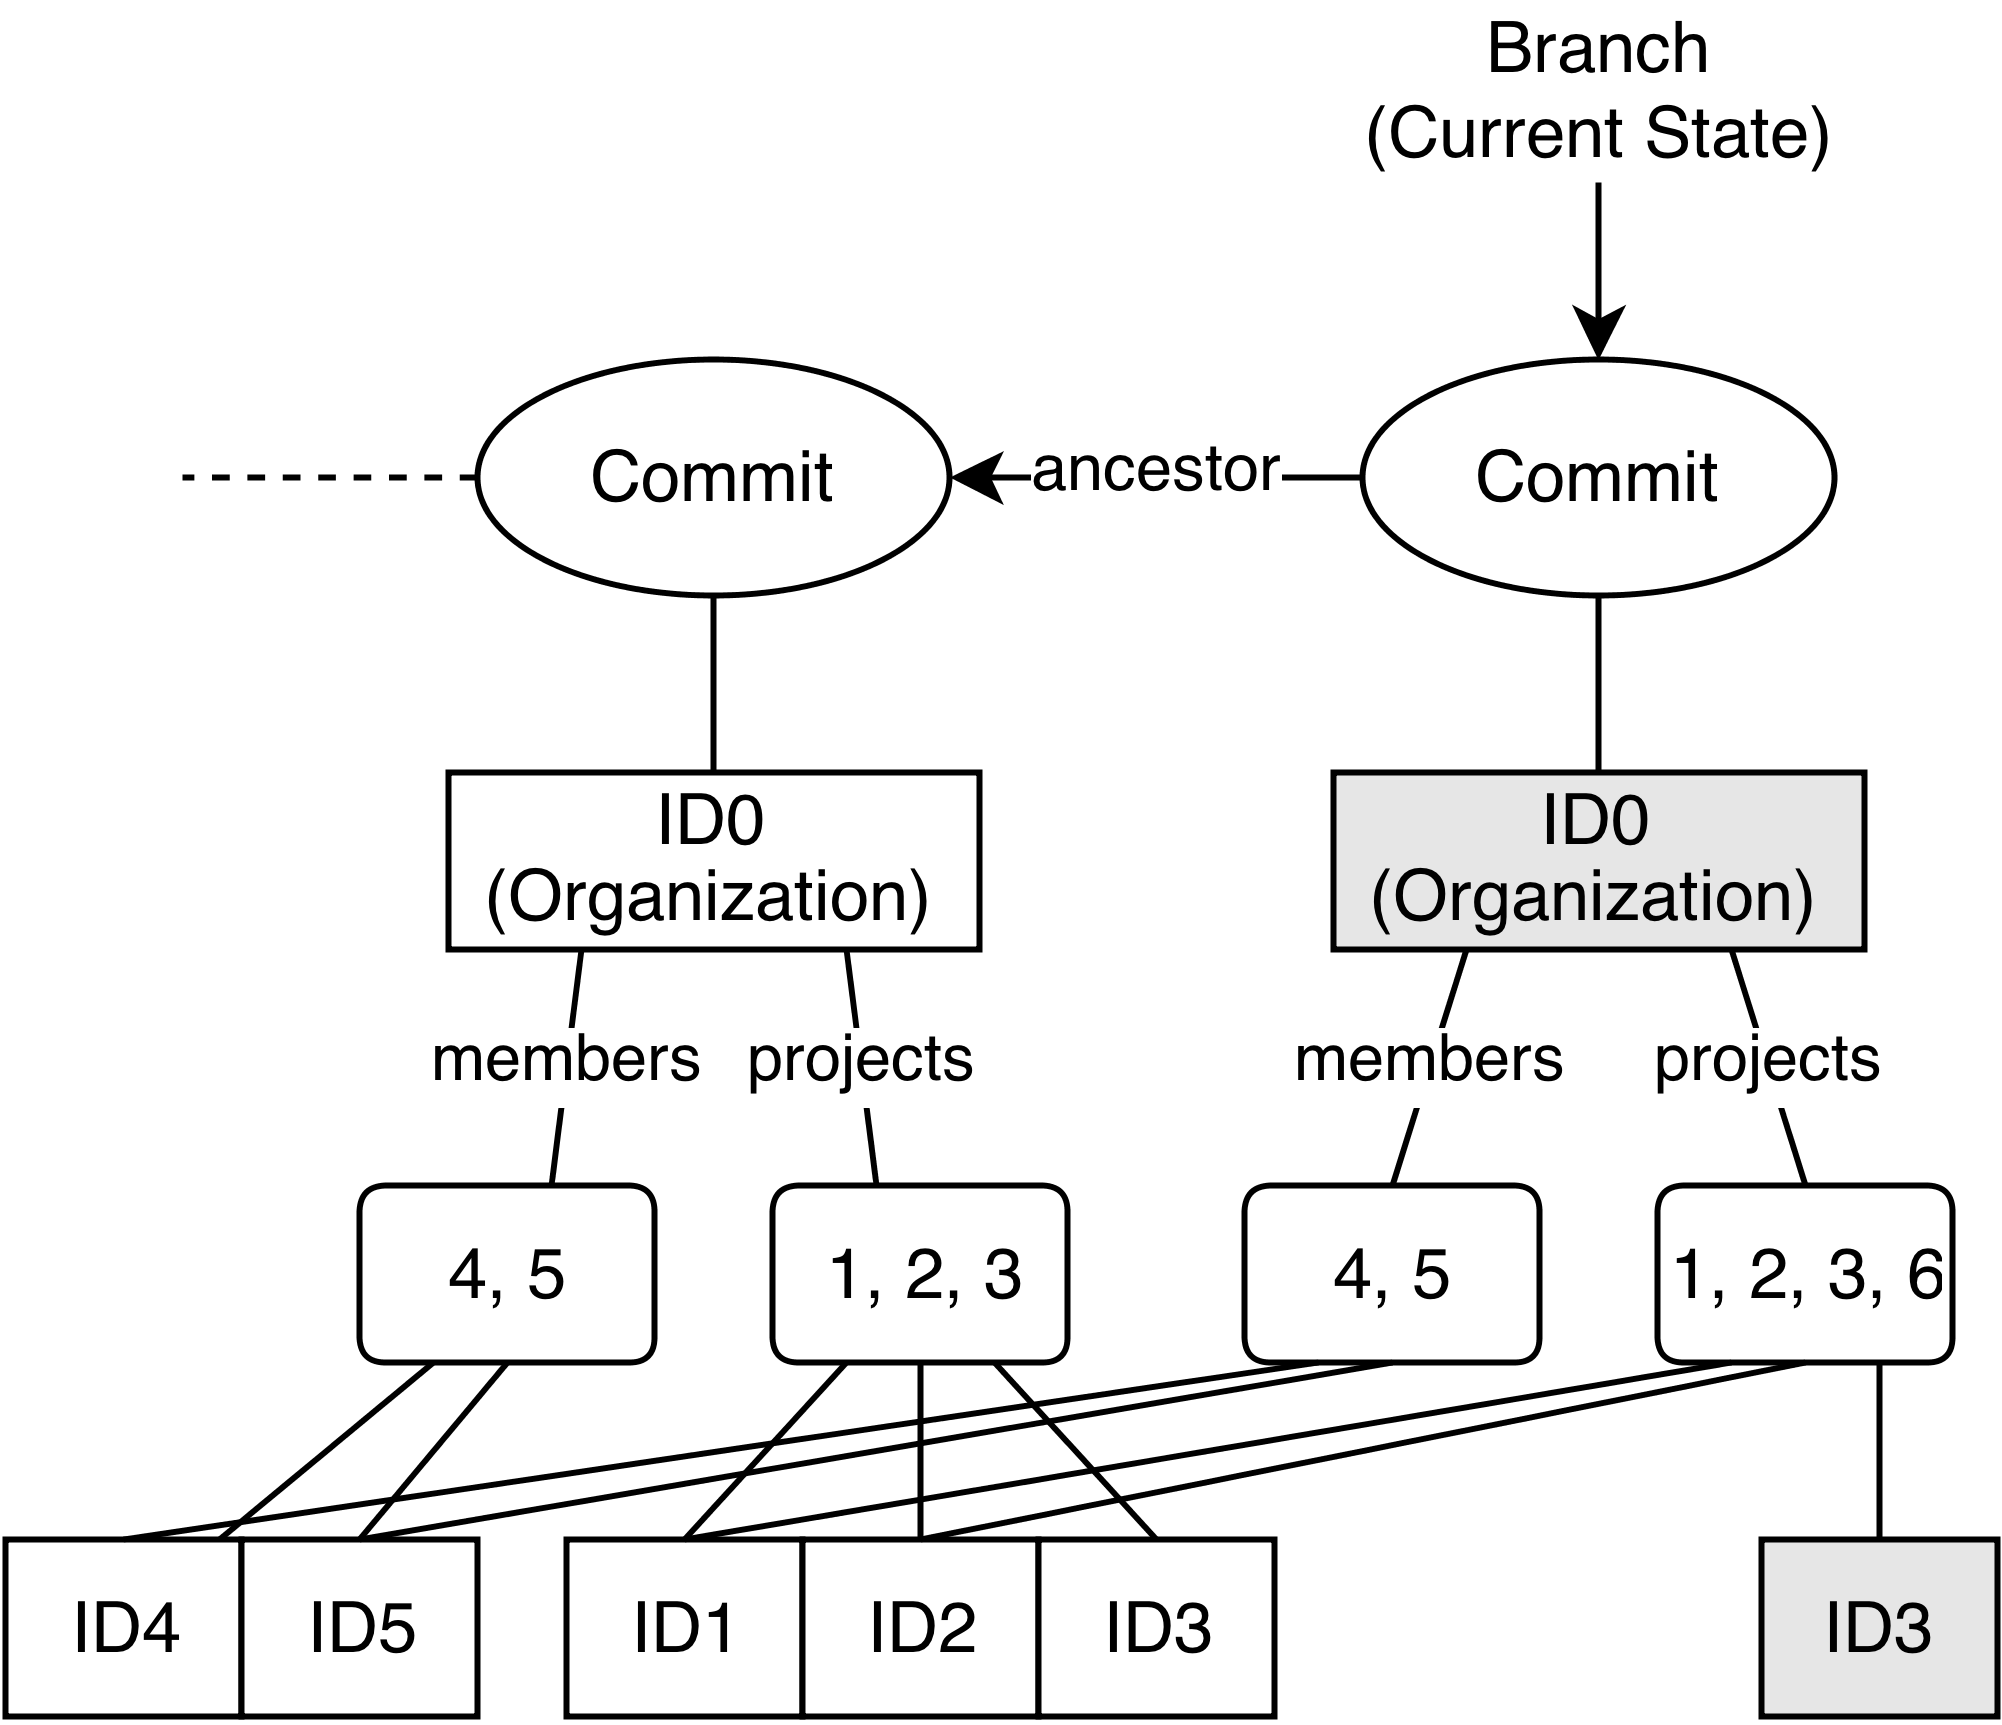
\includegraphics[width=0.6\textwidth]{img/commits}
  \caption{Re-using objects across commits.}
  \label{fig:histo.commits}
\end{figure}

With this model of hierarchical data at hand we can now go into the details of merging two branches of our state.
